\section{Using Parameterizations to Calculate Line Integrals} \label{S:12.3.ParamLineIntegrals}


\vspace*{-14 pt}
\framebox{\hspace*{3 pt}
\parbox{6.25 in}{\begin{goals}
\item How can we use a parameterization of an oriented curve $C$ to
  calculate $\int_C\vF\cdot d\vr$?
\item If a parameterization is used to calculate $\int_C\vF\cdot
  d\vr$, does the parameterization chosen alter the value of the line integral?
\end{goals}} \hspace*{3 pt}}

\subsection*{Introduction}

We begin this section by taking a look at how we might go about
calculating a line integral of a vector field along some line segments
and will use this as inspiration to see how treating oriented curves
as vector-valued functions can allow us to quickly turn a line
integral of a vector field into an integral of a single variable. 

\begin{pa} \label{PA:12.3}
Let $\vF=\langle xy,y^2\rangle$, let $C_1$ be the line segment from
from $(1,1)$ to $(4,1)$, let $C_2$ be the line segment from $(4,1)$ to
$(4,3)$, and let $C_3$ be the line segment from $(1,1)$ to
$(4,3)$. Also let $C = C_1 + C_2$. This vector field and the curves
are shown in Figure~\ref{F:12.3.field-segments}.
\begin{figure}
  \centering
  \begin{overpic}[width=0.55\linewidth]{fig_12_3_preview_field_segments.pdf}
    \put(130,60){$C_1$}
    \put(195,115){$C_2$}
    \put(120,143){$C_3$}
  \end{overpic}
  \caption{A vector field $\vF$ and three oriented curves.}
  \label{F:12.3.field-segments}
\end{figure}

\ba
\item Every point along $C_1$ has $y=1$. Therefore, along $C_1$, the
  vector field $\vF$ can be viewed purely as a function of $x$. In
  particular, along $C_1$, we have $\vF(x,1) = \langle
  x,1\rangle$.
  Since every point along $C_2$ has the same $x$-value, what (in terms
  of $y$ only) is $\vF$ along $C_2$?
\item Recall that $d\vr \approx \Delta \vr$, and along $C_1$, we have
  that $\Delta\vr = \Delta x\vi \approx dx\vi$. Thus, $d\vr = \langle
  dx,0\rangle$. We know that along $C_1$, $\vF = \langle
  x,1\rangle$. What does this mean $\vF\cdot d\vr$ is along $C_1$?
  What interval of $x$-values describes $C_1$? Use these facts
  fact to write $\int_{C_1} \vF\cdot d\vr$ as an integral of the form
  $\int_a^b f(x)\, dx$ and evaluate the integral. 
\item Use an analogous approach to write $\int_{C_2} \vF\cdot d\vr$ as
  a limit of the form $\int_\alpha^\beta g(y)\, dy$ and evaluate the
  integral.
\item Use the previous parts and a property of line integrals to
  calculate $\int_C\vF\cdot d\vr$ without having to evaluate any
  additional integrals. 
\item Evaluating $\int_{C_3}\vF\cdot d\vr$ takes more work at this
  stage, so let's break the process into smaller pieces.
  \begin{enumerate}[label=\roman*.]
\label{F:12.3.field-segments}  \item Since $C_3$ is a line segment, find the slope-intercept
    ($y=mx+b$) form of the equation of this line.
  \item Just as we noticed that along $C_1$ we always had $y=1$, we
    now know how to express $y$ in terms of $x$ for all points along
    $C_3$. Use this to to express $\vF(x,y) = \vF(x,mx+b)$ as a
    vector purely in terms of $x$ for points along $C_3$.
  \item We often think of the slope of a line as being $\Delta
    y/\Delta x$. Use this fact and the slope of the line containing
    $C_3$ to express $\Delta y$ as a multiple of $\Delta x$. 
  \item We may view $\Delta\vr$ as $\langle \Delta x,\Delta y\rangle$.
    Since $\Delta x\approx dx$ and $\Delta y\approx dy$,
    write $d\vr$ as a vector in terms of $dx$.
  \item Use the range of $x$-values covered by the line segment $C_3$
    to write $\int_{C_3}\vF\cdot d\vr$ as a single-variable integral
    of the form $\int_a^b f(x)\, dx$ and evaluate the integral.
  \end{enumerate}
\item Notice that $C$ and $C_3$ both start at $(1,1)$ and end at
  $(4,3)$. How do the values of $\int_C\vF\cdot d\vr$ and
  $\int_{C_3}\vF\cdot d\vr$ compare?
\item Is $\vF$ a gradient vector field? Why or why not?\emph{Hint}: If
  $\vF$ were a gradient vector field, then there would be a function
  $f$ such that $\vF = \nabla f$. What would Clairaut's theorem say in
  this case?
\ea
\end{pa} 
\afterpa 
%%% Local Variables:
%%% mode: latex
%%% TeX-master: "../0_AC_MV"
%%% End:


\subsection*{Parameterizations in the Definition of $\int_C\vF\cdot d\vr$}

Preview Activity~\ref{PA:12.3} has shown us that it is possible to
evaluate line integrals without needing to resort to working with
Riemann sums directly. However, the approaches taken there seem rather
cumbersome to use for oriented curves that are not line
segments. Fortunately, parameterizing the oriented curve along which a
line integral is calculated provides a powerful tool for evaluating
line integrals.

Suppose that $C$ is an oriented curve traced out by the vector-valued
function $\vr(t)$ for $a\leq t\leq b$, and let $\vF$ be a continuous
vector field defined near $C$. We can divide the interval $[a,b]$ into $n$
subintervals, each of length $\Delta t = (b-a)/n$, by letting $t_i = a
+ i\Delta t$ for $i = 0,1,\dots,n$. This subdivision of $[a,b]$ then
can be used to break $C$ up into $n$ pieces by letting $\Delta \vr_i =
\vr(t_{i+1}) - \vr(t_{i})$ for $i=0,1,\dots,n-1$.  Now notice that
\[\Delta \vr_i = \vr(t_{i+1}) - \vr(t_{i}) = \vr(t_{i} + \Delta t) -
\vr(t_{i}) = \frac{\vr(t_{i} + \Delta t) -
\vr(t_{i})}{\Delta t}\Delta t.\]
Since the ratio in the last expression for $\Delta \vr_i$ is
approximately $\vr'(t_{i})$, we can say that $\Delta\vr_i\approx
\vr'(t_i)\Delta t$. Substituting this into the Reimann sum in the
definition of the line integral, we have
      \[\int_C \vF\cdot d\vr = \lim_{|\Delta\vr_i|\to 0}
      \sum_{i=0}^{n-1}\vF(\vr_i)\cdot\Delta\vr_i = \lim_{\Delta t\to
        0} \sum_{i=0}^{n-1} \vF(\vr(t_i))\cdot \vr'(t_i)\Delta t.\]
This final Riemann sum is $\int_a^b \vF(\vr(t))\cdot \vr'(t)\, dt$,
allowing us to reduce the evaluation of a line integral of a
vector-valued function along an oriented curve to an ordinary integral
of a function of one variable, since after evaluating the dot product,
$\vF(\vr(t))\cdot \vr'(t)$ is (scalar) function of $t$. We restate
this result below for easy reference.


\vspace*{5pt}
\nin \framebox{\hspace*{3 pt}
  \parbox{6.25
    in}{\label{thm:12.3.line-integral-evaluation}
      Let $C$ be a smooth, oriented curve traced out by the
      vector-valued function $\vr(t)$ for $a\leq t\leq b$ and let
      $\vF$ be a continuous vector field defined near $C$. Then
      \[\int_C \vF\cdot d\vr = \int_a^b \vF(\vr(t))\cdot \vr'(t)\, dt.\]
      
} \hspace*{3 pt}} \vspace*{5pt}

\begin{example}
  Let $\vF(x,y) = x\vi + y^2\vj$ and let $C$ be the quarter of the circle of
  radius $3$ from $(0,3)$ to $(3,0)$. This vector field and curve are
  shown in Figure~\ref{F:12.3.field-quarter-circle}. By properties of line integrals,
  we know that $\int_C \vF\cdot d\vr = -\int_{-C}\vF\cdot d\vr$, and
  we will use this property since $-C$ is the usual clockwise
  orientation of a circle, meaning we can parameterize $-C$ by $\vr(t)
  = \langle 3\cos(t),3\sin(t)\rangle$ for $0\leq t\leq \pi/2$.
  \begin{figure}
    \centering
    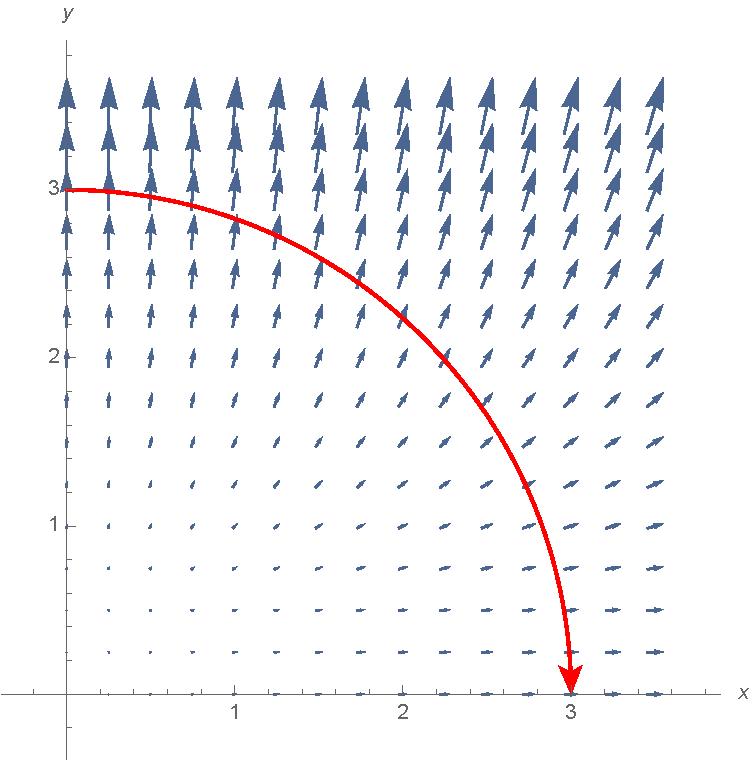
\includegraphics[width=0.4\linewidth]{fig_12_3_field_quarter_circle.pdf}
    \caption{The vector field $\vF = x\vi + y^2\vj$ and an oriented
      curve $C$}
    \label{F:12.3.field-quarter-circle}
  \end{figure}

  To evaluate $\int_{-C}\vF\cdot d\vr$ using this parameterization, we
  need to note that
  \[\vF(\vr(t)) = \langle 3\cos(t) , 9\sin^2(t)\rangle\qquad\text{and}
  \vr'(t) = \langle -3\sin(t),3\cos(t)\rangle.\]
  Thus, we have
  \begin{align*}\int_C\vF\cdot d\vr &= -\int_{-C}\vF\cdot d\vr = -\int_0^{\pi/2}
  \langle 3\cos(t),9\sin^2(t)\rangle\cdot\langle
  -3\sin(t),3\cos(t)\rangle\, dt\\
    &= -\int_0^{\pi/2} \left(-9\sin(t)\cos(t) +
      27\sin^2(t)\cos(t)\right)\, dt\\
    & = -\int_0^1 (-9 u + 27u^2)\, du = -\left[ -\frac{9}{2}u^2 +
      9u^3\right]_0^1 = -\left(-\frac{9}{2} + 9\right) = -\frac{9}{2}.
\end{align*}
\end{example}

\begin{activity} \label{A:12.3.1}  
\ba
\item Find the work done by the vector field
  $\vF(x,y,z) = 6x^2z\vi + 3y^2\vj + x\vk$ on a particle that moves
  from the point $(3,0,0)$ to the point $(3,0,6\pi)$ along the helix
  given by $\vr(t) = \langle 3\cos(t),3\sin(t),t\rangle$.
\item Let $\vF(x,y) = \langle 0,x\rangle$. Let $C$ be the closed curve
  consisting of the top half of the circle of radius $2$ centered at
  the origin and the portion of the $x$-axis from $(2,0)$ to $(-2,0)$,
  oriented clockwise. Find the circulation of $\vF$ around $C$.
\ea
\end{activity}
\begin{smallhint}

\end{smallhint}
\begin{bighint}

\end{bighint}
\begin{activitySolution}

\end{activitySolution}
\aftera
%%% Local Variables:
%%% mode: latex
%%% TeX-master: "../0_AC_MV"
%%% End:


\begin{activity} \label{A:12.3.2}  
\nin Let $\vF(x,y) = \langle y^2,2xy+3\rangle$.
\ba
\item Let $C_1$ be the portion of the graph of $y=x^3-x$ from $(1,0)$
  to $(-1,0)$. Calculate $\int_{C_1}\vF\cdot d\vr$.
\item Let $C_2$ be the line segment from $(1,0)$ to
  $(-1,0)$. Calculate $\int_{C_2}\vF\cdot d\vr$.
\item Let $C_3$ be the circle of radius $3$ centered at the origin,
  oriented counterclockwise. Calculate $\oint_{C_3} \vF\cdot d\vr$.
\ea
\end{activity}
\begin{smallhint}

\end{smallhint}
\begin{bighint}

\end{bighint}
\begin{activitySolution}

\end{activitySolution}
\aftera
%%% Local Variables:
%%% mode: latex
%%% TeX-master: "../0_AC_MV"
%%% End:


\subsection*{Alternative Notation for Line Integrals}

In contexts where the fact that the quantity we are measuring via a
line integral is best measured via a dot product (such as calculating
work), the notation we have used thus far for line integrals is fairly
common. However, sometimes the vector field is such that the units on
$x$, $y$, and $z$ are not distances. In this case, a dot product may
not have a physical meaning, and an alternative notation using
differentials can be common. Specifically, if $\vF(x,y,z) =
F_1(x,y,z)\vi + F_2(x,y,z)\vj + F_3(x,y,z)\vk$, then
\[\int_C\vF\cdot d\vr = \int_C F_1\, dx + F_2\, dy + F_3\, dz.\]
(If $\vF$ is a vector field in $\R^2$, the $F_3\, dz$ term is
omitted.) As a concrete example, if $\vF(x,y,z) = \langle
x^2y,z^3,x\cos(z)\rangle$ and $C$ is some oriented curve in $\R^3$,
then
\[\int_C\vF\cdot d\vr = \int_C x^2y\, dx + z^3\, dy + x\cos(z)\, dz.\]
It is important to recognize that the integral on the right-hand side
is still a line integral and must be evaluated using techniques for
evaluating line integrals. We cannot simply try to treat it as if it
were a definite integral of a function of one variable.

\subsection*{Independence of Parameterization}

Up to this point, we've just been choosing whatever parameterization
of an oriented curve $C$ came to mind, and our argument for how we can
use parameterizations to calculate line integrals did not depend on
the specific choice of parameterization. However, it is not
immediately obvious that different parameterizations don't result in
different values of the line integral. Our next example explores this question.

\begin{example}\label{ex:12.3.param-indep}
  Consider the vector field $\vF = x\vi$. Let us consider two
  different oriented curves from $(0,1)$ to $(3,3)$. The first
  oriented curve $C$ travels horizontally to $(3,1)$ and then proceeds
  vertically to $(3,3)$. The second oriented curve $C_3$ is the line
  segment from $(0,1)$ to $(3,3)$. Notice that, as depicted in
  Figure~\ref{F:12.3.x-field-triangle}, we can break $C$ up into two
  oriented curves $C_1$ (the horizontal portion) and $C_2$ (the
  vertical portion) so that $C = C_1 + C_2$.
  \begin{figure}
    \centering
    \begin{overpic}[width=0.4\linewidth]{figures/fig_12_3_field_triangle.pdf}
      \put(80,48){$C_1$}
      \put(150,92){$C_2$}
      \put(80,115){$C_3$}
    \end{overpic}
    \caption{The vector field $\vF = x\vi$ and some oriented curves.     \label{F:12.3.x-field-triangle}}

  \end{figure}
  
  We first note that since $\vF$ is orthogonal to $C_2$,
  $\int_{C_2}\vF\cdot d\vr=0$; threfore $\int_C\vF\cdot d\vr =
  \int_{C_1}\vF\cdot d\vr$. We can parameterize $C_1$ as just $x\vi+\vj$
  for $0\leq x\leq 3$, which leads to
  \[\int_{C_1}\vF\cdot d\vr = \int_0^3\langle x,0\rangle\cdot \langle
  1,0\rangle\, dx = \int_0^3 x\, dx = \frac{9}{2}.\]
  Thus, $\int_C\vF\cdot d\vr = 9/2$.

  Now we look at $\int_{C_3}\vF\cdot d\vr$, but we parameterize $C_3$
  in a bit of a nonstandard way by letting $\vr(t) = \langle
  3\sin(t),1+2\sin(t)\rangle$ for $0\leq t\leq \frac{\pi}{2}$. Then
  $\vr'(t) = \langle 3\cos(t),2\cos(t)\rangle$, and
  \[\int_{C_3}\vF\cdot d\vr = \int_0^{\pi/2}\langle
  3\sin(t),0\rangle\cdot\langle 3\cos(t),2\cos(t)\rangle\, dt =
  \int_0^{\pi/2} 9\sin(t)\cos(t)\, dt = \frac{9}{2}.\]
  In the next activity, you are asked to consider the more typical
  parameterization of $C_3$ and verify that using it gives the same
  value for the line integral.

  It's also worth observing here that $\int_C\vF\cdot d\vr =
  \int_{C_3}\vF\cdot d\vr$, so at least two (very different) paths
  from $(0,1)$ to $(3,3)$ give the same value of the line integral
  here. The next section will further investigate this phenomenon and
  when it happens.
\end{example}

\begin{activity} \label{A:12.3.3}  
\ba
\item The typical parameterization of the line segment from $(0,1)$ to
  $(3,3)$ (the oriented curve $C_3$ in
  Example~\ref{ex:12.3.param-indep}) is $\vr(t) = \langle 3t,1+2t\rangle$. Use this
  parameterization to calculate $\int_{C_3}\vF\cdot d\vr$ for the
  vector field $\vF = x\vi$.
\item Calculate $\int_C (3xy+e^z)\, dx + x^2\, dy + (4z+xe^z)\, dz$
  where $C$ is the oriented curve consisting of the line segment from
  the origin to $(1,1,1)$ followed by the line segment from $(1,1,1)$
  to $(0,0,2)$.
\item Calculate $\int_{C'} (3xy+e^z)\, dx + x^2\, dy + (4z+xe^z)\, dz$
  where $C'$ is the line segment from $(0,0,0)$ to $(0,0,2)$.
\ea
\end{activity}
\begin{smallhint}

\end{smallhint}
\begin{bighint}

\end{bighint}
\begin{activitySolution}

\end{activitySolution}
\aftera
%%% Local Variables:
%%% mode: latex
%%% TeX-master: "../0_AC_MV"
%%% End:


%\nin \framebox{\hspace*{3 pt}
%\parbox{6.25 in}{
\begin{summary}
\item If $C_1$ and $C_2$ are different paths from $P$ to $Q$, it is
  possible for $\int_{C_1}\vF\cdot d\vr$ to have a different value to
  $\int_{C_2}\vF\cdot d\vr$.
\item Line integrals of vector fields along oriented curves can be
  evaluated by parameterizing the curve in terms of $t$ and then
  calculating the integral of $\vF(\vr(t))\cdot \vr'(t)$ on the
  interval $[a,b]$.
\item The line integral $\int_C\vF\cdot d\vr$ can also be written as
  $\int_C F_1\, dx + F_2\, dy$ if $\vF = \langle F_1,F_2\rangle$ is a
  vector field in $\R^2$ or $\int_C F_1\, dx + F_2\, dy + F_3\, dz$ if
  $\vF = \langle F_1,F_2,F_3\rangle$ is a vector field in $\R^3$.
\end{summary}
%} \hspace*{3 pt}}

\nin \hrulefill

%\input{exercises/9.2.Vectors(Ex)}

\clearpage

%%% Local Variables:
%%% mode: latex
%%% TeX-master: "0_AC_MV"
%%% End:
